\subsection{All new results and exact run identities}
All results below use 2,070 test clips. Text only, Visual+text, and Text+text use descriptions; all other rows use visual input. Every listed run completed with exit 0:0.
\begingroup\footnotesize\setlength{\tabcolsep}{4pt}
\begin{longtable}{lrrrrrrr}
\caption{The 34 new benchmark conditions. Names ending in a number specify K; perm. denotes the fixed semantic-permutation control.}\\
\toprule
Model & KL $\downarrow$ & Cos $\uparrow$ & Inter $\uparrow$ & Cheb $\downarrow$ & MRR $\uparrow$ & F1@1 $\uparrow$ & F1@3 $\uparrow$\\\midrule\endhead
VAD aux & 0.54987 & 0.82260 & 0.63694 & 0.22164 & 0.72750 & 0.53318 & 0.60804\\
VAD aux perm. & 0.54722 & 0.82382 & 0.63700 & 0.22075 & 0.72658 & 0.53504 & 0.60734\\
VAD geom. & 0.54278 & 0.82589 & 0.63168 & 0.22380 & 0.72874 & 0.53458 & 0.61941\\
VAD geom. perm. & 0.54693 & 0.82286 & 0.63147 & 0.22374 & 0.72547 & 0.53702 & 0.61499\\
C logits & 0.55503 & 0.81977 & 0.62951 & 0.22535 & 0.71885 & 0.52600 & 0.62017\\
C VAD & 0.54631 & 0.82366 & 0.63333 & 0.22252 & 0.72230 & 0.53005 & 0.61599\\
C both & 0.54817 & 0.82318 & 0.63471 & 0.22141 & 0.72735 & 0.54057 & 0.61195\\
F global+peak & 0.55644 & 0.82114 & 0.63194 & 0.22340 & 0.72431 & 0.53173 & 0.60059\\
F global+global & 0.54604 & 0.82416 & 0.63022 & 0.22498 & 0.72932 & 0.54245 & 0.61418\\
F peak+peak & 0.59209 & 0.80357 & 0.61555 & 0.23607 & 0.70131 & 0.49647 & 0.58987\\
D arousal 4 & 0.58272 & 0.80358 & 0.61518 & 0.23521 & 0.69614 & 0.48266 & 0.59361\\
D distance 4 & 0.58235 & 0.80494 & 0.61615 & 0.23478 & 0.70468 & 0.49038 & 0.59219\\
D confidence 4 & 0.58148 & 0.80637 & 0.61469 & 0.23531 & 0.70394 & 0.49254 & 0.59629\\
D uniform 4 & 0.57179 & 0.80821 & 0.61808 & 0.23431 & 0.70426 & 0.49814 & 0.59732\\
D random 4 & 0.57872 & 0.80670 & 0.61743 & 0.23355 & 0.70111 & 0.49360 & 0.59161\\
Text only & 0.54943 & 0.81224 & 0.62545 & 0.23254 & 0.70705 & 0.50303 & 0.60958\\
Visual+text & 0.50995 & 0.83802 & 0.64647 & 0.21324 & 0.74790 & 0.56332 & 0.62590\\
Visual+visual & 0.54742 & 0.82567 & 0.63879 & 0.21929 & 0.73012 & 0.54279 & 0.61390\\
Text+text & 0.55149 & 0.81179 & 0.62211 & 0.23420 & 0.70491 & 0.50413 & 0.60932\\
D arousal 1 & 0.62134 & 0.78626 & 0.59354 & 0.25045 & 0.67237 & 0.44690 & 0.58272\\
D distance 1 & 0.62214 & 0.78602 & 0.59998 & 0.24686 & 0.67026 & 0.44577 & 0.58250\\
D confidence 1 & 0.62240 & 0.78462 & 0.59813 & 0.24787 & 0.67647 & 0.44704 & 0.57961\\
D uniform 1 & 0.60659 & 0.79666 & 0.60394 & 0.24277 & 0.69043 & 0.48107 & 0.58653\\
D random 1 & 0.61068 & 0.79267 & 0.60529 & 0.24416 & 0.66895 & 0.44757 & 0.58158\\
D arousal 2 & 0.59945 & 0.79751 & 0.60483 & 0.24237 & 0.69018 & 0.47144 & 0.58919\\
D distance 2 & 0.60555 & 0.79178 & 0.60668 & 0.24224 & 0.68078 & 0.45121 & 0.58286\\
D confidence 2 & 0.59899 & 0.79801 & 0.60570 & 0.24090 & 0.68591 & 0.46167 & 0.58739\\
D uniform 2 & 0.59077 & 0.80308 & 0.61142 & 0.23749 & 0.70129 & 0.49762 & 0.59207\\
D random 2 & 0.59490 & 0.79955 & 0.61120 & 0.23943 & 0.69525 & 0.48431 & 0.59750\\
D arousal 8 & 0.56374 & 0.81521 & 0.62666 & 0.22940 & 0.71795 & 0.52036 & 0.61406\\
D distance 8 & 0.56662 & 0.81476 & 0.63032 & 0.22691 & 0.71467 & 0.51706 & 0.60277\\
D confidence 8 & 0.56602 & 0.81418 & 0.62350 & 0.22956 & 0.71128 & 0.50947 & 0.60315\\
D uniform 8 & 0.55799 & 0.81942 & 0.62504 & 0.22857 & 0.72108 & 0.52713 & 0.61533\\
D random 8 & 0.56370 & 0.81463 & 0.62358 & 0.23065 & 0.71078 & 0.50190 & 0.60348\\
\bottomrule\end{longtable}\endgroup

\begingroup\footnotesize\setlength{\tabcolsep}{4pt}
\begin{longtable}{lrrrr}
\caption{Remaining official metrics for every new condition.}\\
\toprule
Model & Clark $\downarrow$ & CAD $\downarrow$ & TPE $\downarrow$ & F1@2 $\uparrow$\\\midrule\endhead
VAD aux & 3.94709 & 2.61618 & 0.18048 & 0.60842\\
VAD aux perm. & 3.94823 & 2.60299 & 0.18013 & 0.60917\\
VAD geom. & 3.94136 & 2.62029 & 0.18968 & 0.61115\\
VAD geom. perm. & 3.94318 & 2.60205 & 0.18973 & 0.60237\\
C logits & 3.93946 & 2.63700 & 0.19006 & 0.60806\\
C VAD & 3.94133 & 2.59936 & 0.18713 & 0.60723\\
C both & 3.94131 & 2.60423 & 0.18225 & 0.60556\\
F global+peak & 3.94926 & 2.62892 & 0.18542 & 0.60331\\
F global+global & 3.93751 & 2.63161 & 0.19204 & 0.60571\\
F peak+peak & 3.95818 & 2.77490 & 0.19887 & 0.58479\\
D arousal 4 & 3.95725 & 2.70612 & 0.19862 & 0.58692\\
D distance 4 & 3.95467 & 2.71322 & 0.19847 & 0.58619\\
D confidence 4 & 3.95046 & 2.70365 & 0.20128 & 0.59386\\
D uniform 4 & 3.95134 & 2.70129 & 0.19907 & 0.58672\\
D random 4 & 3.95334 & 2.72013 & 0.19782 & 0.58629\\
Text only & 3.94605 & 2.67450 & 0.19789 & 0.59792\\
Visual+text & 3.94036 & 2.49565 & 0.17838 & 0.61834\\
Visual+visual & 3.93911 & 2.58417 & 0.17891 & 0.61081\\
Text+text & 3.94290 & 2.70874 & 0.20221 & 0.59528\\
D arousal 1 & 3.95186 & 2.91944 & 0.21944 & 0.56572\\
D distance 1 & 3.96003 & 2.86059 & 0.21059 & 0.56363\\
D confidence 1 & 3.96006 & 2.86694 & 0.21372 & 0.56124\\
D uniform 1 & 3.95699 & 2.86026 & 0.21024 & 0.57387\\
D random 1 & 3.96075 & 2.83078 & 0.21065 & 0.55822\\
D arousal 2 & 3.95247 & 2.81884 & 0.20983 & 0.57228\\
D distance 2 & 3.95990 & 2.78935 & 0.20621 & 0.57409\\
D confidence 2 & 3.95500 & 2.82950 & 0.20936 & 0.57285\\
D uniform 2 & 3.95653 & 2.81425 & 0.20266 & 0.57915\\
D random 2 & 3.95937 & 2.77174 & 0.20365 & 0.57403\\
D arousal 8 & 3.94247 & 2.67593 & 0.19334 & 0.60383\\
D distance 8 & 3.95356 & 2.65023 & 0.18328 & 0.59925\\
D confidence 8 & 3.94818 & 2.66753 & 0.19347 & 0.60103\\
D uniform 8 & 3.94172 & 2.66397 & 0.19598 & 0.59673\\
D random 8 & 3.94735 & 2.68565 & 0.19552 & 0.59142\\
\bottomrule\end{longtable}\endgroup

\begingroup\footnotesize\setlength{\tabcolsep}{4pt}
\begin{longtable}{lrrrrr}
\caption{New run identities and validation-only checkpoint selection. All use frozen source 99b59ad.}\\
\toprule
Model & Job ID & Parameters & Best epoch & Epochs & Val KL\\\midrule\endhead
VAD aux & 27612811 & 169,496 & 8 & 16 & 0.543622\\
VAD aux perm. & 27612813 & 169,496 & 8 & 16 & 0.543786\\
VAD geom. & 27612816 & 169,109 & 9 & 17 & 0.542680\\
VAD geom. perm. & 27612819 & 169,109 & 12 & 20 & 0.541011\\
C logits & 27612828 & 170,517 & 12 & 20 & 0.548607\\
C VAD & 27612829 & 170,517 & 12 & 20 & 0.541462\\
C both & 27612830 & 170,517 & 8 & 16 & 0.547655\\
F global+peak & 27612832 & 185,493 & 7 & 15 & 0.556795\\
F global+global & 27612834 & 185,493 & 9 & 17 & 0.547622\\
F peak+peak & 27612836 & 185,493 & 7 & 15 & 0.594158\\
D arousal 4 & 27612842 & 169,109 & 5 & 13 & 0.590107\\
D distance 4 & 27612844 & 169,109 & 5 & 13 & 0.588314\\
D confidence 4 & 27612847 & 169,109 & 5 & 13 & 0.587223\\
D uniform 4 & 27612848 & 169,109 & 5 & 13 & 0.577427\\
D random 4 & 27612849 & 169,109 & 5 & 13 & 0.582785\\
Text only & 27612851 & 169,109 & 2 & 10 & 0.547431\\
Visual+text & 27612852 & 335,381 & 2 & 10 & 0.510391\\
Visual+visual & 27612854 & 335,381 & 10 & 18 & 0.548417\\
Text+text & 27612856 & 335,381 & 2 & 10 & 0.551836\\
D arousal 1 & 27614365 & 169,109 & 2 & 10 & 0.627894\\
D distance 1 & 27614367 & 169,109 & 5 & 13 & 0.624926\\
D confidence 1 & 27614368 & 169,109 & 5 & 13 & 0.618938\\
D uniform 1 & 27614371 & 169,109 & 2 & 10 & 0.617071\\
D random 1 & 27614372 & 169,109 & 3 & 11 & 0.619144\\
D arousal 2 & 27614373 & 169,109 & 2 & 10 & 0.608466\\
D distance 2 & 27614374 & 169,109 & 5 & 13 & 0.610554\\
D confidence 2 & 27614375 & 169,109 & 2 & 10 & 0.603221\\
D uniform 2 & 27614376 & 169,109 & 2 & 10 & 0.597875\\
D random 2 & 27614377 & 169,109 & 3 & 11 & 0.595427\\
D arousal 8 & 27614378 & 169,109 & 9 & 17 & 0.571545\\
D distance 8 & 27614379 & 169,109 & 8 & 16 & 0.568878\\
D confidence 8 & 27614380 & 169,109 & 5 & 13 & 0.569350\\
D uniform 8 & 27614381 & 169,109 & 9 & 17 & 0.558642\\
D random 8 & 27614382 & 169,109 & 5 & 13 & 0.563106\\
\bottomrule\end{longtable}\endgroup

\subsection{Controlled comparisons and interpretation}
\begingroup\footnotesize\setlength{\tabcolsep}{4pt}
\begin{longtable}{lrl}
\caption{Predeclared model/control comparisons. Negative values favor the first model. Intervals use 10,000 paired movie resamples, one training seed, and no multiplicity correction.}\\
\toprule
Comparison & $\Delta$ KL & 95\% movie-bootstrap interval\\\midrule\endhead
Visual+text minus B1 & -0.034462 & [-0.042130, -0.027175]\\
Visual+text minus Text only & -0.039480 & [-0.045894, -0.033091]\\
Visual+text minus Visual+visual & -0.037467 & [-0.045994, -0.029385]\\
Visual+text minus Text+text & -0.041542 & [-0.047972, -0.035109]\\
VAD aux minus B1 & +0.005451 & [+0.000756, +0.010088]\\
VAD aux minus VAD aux perm. & +0.002645 & [+0.000953, +0.004350]\\
VAD geom. minus B1 & -0.001637 & [-0.003355, +0.000050]\\
VAD geom. minus VAD geom. perm. & -0.004154 & [-0.008003, -0.000237]\\
F global+peak minus F global+global & +0.010404 & [+0.004587, +0.016331]\\
F global+peak minus F peak+peak & -0.035645 & [-0.041536, -0.029633]\\
\bottomrule\end{longtable}\endgroup

\textbf{Descriptions add complementary information.} Visual+text lowers KL from B1\textquotesingle s 0.544414 to 0.509952, a 6.33\% relative reduction. It improves over both equally sized controls, so increased capacity alone does not explain the gain. Text only is inconclusive against B1. This supports complementarity for this frozen representation and official split, not label leakage or universal text superiority.
\textbf{VAD is not a demonstrated baseline improvement.} Auxiliary regression worsens KL relative to B1 and its own semantic control. Geometry regularization improves over its permuted control, but its B1 interval reaches +0.000050. Moreover, expected-VAD squared error is 0.039762 for sourced geometry versus 0.039529 for its control and 0.039869 for B1; the control has the slightly better affect-space point estimate. These post-hoc diagnostics do not establish fewer affectively implausible errors.
\textbf{Extra frame-emotion features do not clearly help.} C logits worsens KL by +0.010617 [0.005767, 0.015373] versus B1. C VAD and C both have worse point estimates with intervals including zero. The proxy emotion model and input projection may limit these comparisons; negative results do not invalidate all affective visual encoders.
\textbf{Global appearance is useful; the tested peak branch does not add value.} F global+peak is better than peak+peak but worse than global+global. Thus, adding broad context rescues part of the peak-only loss, while the selected peak representation does not improve the matched global predictor. The model uses order-independent pooling and does not test narrative comprehension.
\subsection{The complete peak grid}
\begin{figure}[!htbp]\centering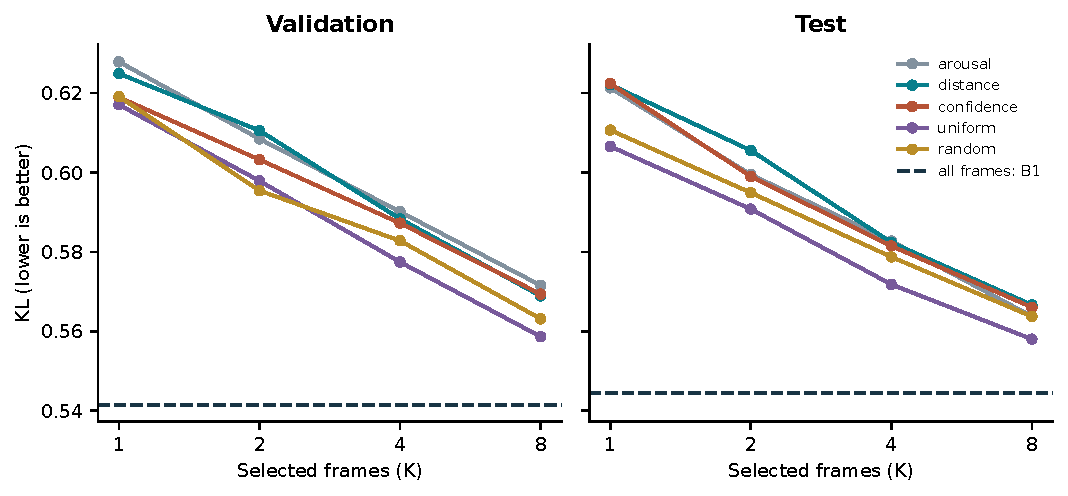
\includegraphics[width=\textwidth]{figures/peak_grid.pdf}
\caption{All declared K values and equal-K controls. Lower KL is better. The dashed line is the shared all-frame B1 reference; no K or score was chosen using test performance.}\end{figure}\FloatBarrier
Every subset has worse test KL than B1, with its paired interval entirely above zero. Uniform selection has lower point-estimate KL than each emotion score at every K. Eleven of the twelve emotion-versus-uniform intervals exclude zero in the unfavorable direction; arousal K=8 is inconclusive. Relative to random selection, several differences are inconclusive and none establishes an affect-ranking advantage. Performance improves as K increases; there is no observed inverted-U favoring sparse emotional peaks. The broader peak hypothesis remains conditional on the quality of these proxy scores.
